%%%%%%%%%%%%%%%%%%%%%%%%%%%%%%%%%%%%%%%%%%%%%%%%%%%%%%%%%%%
% --------------------------------------------------------
% Rho
% LaTeX Template
% Version 2.0.0 (21/05/2024)
%
% Authors: 
% Guillermo Jimenez (memo.notess1@gmail.com)
% Eduardo Gracidas (eduardo.gracidas29@gmail.com)
% 
% License:
% Creative Commons CC BY 4.0
% --------------------------------------------------------
%%%%%%%%%%%%%%%%%%%%%%%%%%%%%%%%%%%%%%%%%%%%%%%%%%%%%%%%%%%

\documentclass[11pt,proc,twoside]{RMxAC_rho-class/RMxAC_rho}

%   ONE PAGE version
%
% Abstract , resumen, corres-info and line numbers should be in false 
\setbool{rho-abstract}{false} % Set false to hide the abstract
\setbool{rho-resumen}{false} % Set false to hide the abstract
\setbool{corres-info}{false} % Set false to hide the corresponding author section
\setbool{linenumbers}{false} % Set false to hide the line numbering

\newcommand\rmaatex{RMxAC}
\newcommand{\CS}[1]{\texttt{\textbackslash #1}}
%----------------------------------------------------------
% volume
%----------------------------------------------------------
\vol{59}
%
\newenvironment{Example}
{\begin{list}{}{\setlength{\leftmargin}{10pt}\setlength{\rightmargin}{10pt}}%
  \item[]\itshape}
  {\end{list}}


%----------------------------------------------------------
% TITLE
%----------------------------------------------------------
%\journalname{\Large Revista Mexicana de Astronomía y Astrofísica 62, 1-10 (2026) \hfill {\includegraphics[width=1.2in, height=0.5in]{LogoRMxAASCamarillo.png}} \\}

\title{ \rmaatex ~ template for Serie de Conferencias preparation  v1.0}

%----------------------------------------------------------
% AUTHORS AND AFFILIATIONS
%----------------------------------------------------------

\author[1,$\dagger$]{Irene~Cruz-González \orcidlink{0000-0002-2653-1120}}
\author[2]{Carlos~G.~ Román-Zúñiga \orcidlink{0000-0001-8600-4798}}
\author[3,$\dagger$]{William~J.~Henney \orcidlink{0000-0001-6208-9109}}
%\author[1,2,$\dagger$]{A. Student}
\author[2,4]{M.~Y.~Posdoc}

%----------------------------------------------------------

\affil[1]{Universidad Nacional Autónoma de México, Instituto de Astronomía, AP 106,  Ensenada 22800, BC, México}
\affil[2]{Universidad Nacional Autónoma de México, Instituto de Radioastronomía y Astrofísica.\\
Antigua Carretera a Pátzcuaro 8701, Ex-Hda. San José de la Huerta, 58089, Morelia, Michoacán, México}
\affil[3]{Universidad Nacional Autónoma de México, Instituto de Astronomía, AP 70-264, CDMX 04510, México}
\affil[4]{One more affiliation you may need}
\affil[$\dagger$]{This project is part of a collaboration/consortium/program}


%----------------------------------------------------------
% DATES
%----------------------------------------------------------

%\dates{This manuscript was compiled on June 25th, 2024}

%----------------------------------------------------------
% FOOTER INFORMATION
%----------------------------------------------------------

\leadauthor{Cruz-González et al.}
% Aquí título de la Conferencia
\smalltitle{{\bf {\it Local Volume Mapper III},
Zihuatanejo, Gro., México, September 10-15 2026
Editors for this issue: Milky Way, Magellanic Cloud \& Messier 33}}

%\institution{Universidad Nacional Autónoma de México}
%\footinfo{Creative Commons CC BY 4.0}
%\theday{November 20th, 2024} %\today

%----------------------------------------------------------
% ARTICLE INFORMATION
%----------------------------------------------------------

\corres{Irene Cruz-González}
\email{icruzgonzalez@astro.unam.mx}

\received{\today}
%\revised{April 16, 2024}
\accepted{April 20, 2025}
%\published{May 21, 2024}
\doi{\url{https://www.astroscu.unam.mx/rmaa/RMxAA..XX-X}}

%\license{Rho LaTeX Class \ccLogo\ This document is licensed under Creative Commons CC BY 4.0.}

%----------------------------------------------------------
% ABSTRACT
%----------------------------------------------------------

%\begin{resumen}
%Este documento (\texttt{rmxaa$\_$SC$\_$example.tex}  (última actualización Febrero, 2025) describe de manera breve el uso de la versión 1.0 de los macros\texttt{\rmaatex} en \LaTeX{}. Provee una guía y un templete común para que los autores puedan preparar sus propios artículos (extenso, breve o resumen) y enviarlos a los Editores Especiales del volumen correspondiente de la Revista Mexicana de Astronomía y Astrofísica Serie de Conferencias. El manuscrito contiene información básica sobre el contenido, así como ejemplos de figuras, tablas y la inclusión de líneas de código o pseudo-código. Se hace uso de la clase rho($\rho$) \LaTeX, especialmente diseñada para propósitos académicos. La guía de usuario (en preparación) contiene detalles adicionales. Se asume que el autor está familiarizado con los rudimentos de \LaTeX{}. En caso de que no sea así, se proveen algunos enlaces útiles en las referencias de la guía de usuario.
%\end{resumen}

%\begin{abstract}
%This document (\texttt{rmxaa$\_$SC$\_$example.tex} (last updated February, 2025) gives a brief tutorial in the use of version 1 of  \texttt{\rmaatex} \LaTeX{} macros. This guide can also serve as  a template for the preparation of papers to be published in  RMxAC. It provides tutorial information and a common template for authors to prepare their conference proceedings contribution (extended, short or abstract) for submission to the Special Editors of the corresponding volume of the Revista Mexicana de Astronomía y Astrofísica Serie de Conferencias. This is an example manuscript.  The manuscript includes basic information about the content, as well as examples for figures, tables and code lines. We are making use of the rho($\rho$) \LaTeX class, specially designed for academic purposes. More details can be found in the user guide (in preparation). It is assumed that the author is already familiar with the rudiments of \LaTeX{}. In case you are not, some suitable references are given in that guiding document.
%\end{abstract}



%----------------------------------------------------------

%\keywords{keyword 1, keyword 2, keyword 3, keyword 4, keyword 5}

%\pclave{palabra clave 1, palabra clave 2, palabra clave 3}

%----------------------------------------------------------

\begin{document}
	
\maketitle
%\pagestyle{fancy}
\thispagestyle{firststyle}
%\tableofcontents

%----------------------------------------------------------




%\section{Introduction}


\begin{rhoenv}[frametitle=Abstract]
   % \boldabstract
    {Welcome to the \rmaatex ~ template, based on the \textit{rho class} style to prepare your contribution to the proceeding of the conference that you atttended to be published in RMxAC. There are three types of macros for contributions for publication in the Serie de Conferencias:  {\it “rm-extenso”, “rm-onepage”} or {\it “rm-shortabstract”}, depending on the case. \\This is the onepage contribution example. Note that the standard Abstract environment is not used and there is no Spanish resumen}
\end{rhoenv}

%The version of the RMxAC\_rho document class described in this User Guide is 1.0 (\today). Its use requires a relatively recent version of \LaTeX{}, although it is optimized to work directly online using \textbf{Overleaf}. The current version of the \LaTeX{} Project Public License is 1.3c (2008). In this guide, some familiarity with the use of \LaTeX{} is assumed. For the author who requires a general introduction to \LaTeX{}, we recommend starting at The LaTeX Project website \url{https://www.latex-project.org/about/}, or using the Overleaf LaTeX guide \url{https://www.overleaf.com/learn/latex/Free_online_introduction_to_LaTeX_(part_1)}. 

Given that you only have one page, you probably don't want to waste
space with frivolities such as section headings.  

The general structure of the flow variables along the symmetry axis of
the bowshock shell is illustrated schematically in
Figure~\ref{fig:simple}.  The approximately isothermal proplyd flow
accelerates from the sound speed up to a Mach number $\mathcal{M}_0$
at the position of the shock. If the number density and temperature
immediately before the shock are $N_0$, $T_0$, then the
Rankine-Hugoniot conditions give the values immediately after
the shock to be \citep{1987flme.book.....L}. %(Landau \& Lifschitz 1987)
\begin{equation}
  \label{eq:mjump}
  \mathcal{M}_1 = \left( \frac{ \mathcal{M}_0^2 + 3 } { 5
      \mathcal{M}_0^2 - 1 } \right)^{1/2} , 
\end{equation}
\begin{equation}
  \label{eq:njump}
  N_1 = \frac{ 4 } { 1 + 3 \mathcal{M}_0^{-2} } N_0 , 
\end{equation}
\begin{equation}
  \label{eq:tjump}
  T_1 = \frac{1}{16} \left( 5 \mathcal{M}_0^2 - 1 \right) 
  \left( 1 + 3 \mathcal{M}_0^{-2} \right) T_0 .
\end{equation}
For instance, using $\mathcal{M}_0 = \mathcal{M}_{A} = 2.7$ from
equation~(99), one obtains $\mathcal{M}_1 = 0.54$,
$N_1 = 2.83 N_0 = 5.77 \times 10^4$\,cm$^{-3}$, $T_1 = 3.13 T_0 =
30,500$\,K, so that the density and temperature jump across the shock
are both roughly a factor of 3.

The emission from the cooling zone behind the shock can be crudely
approximated as the emission from a homogeneous layer with density
$N_1$ and temperature $T_1$ and with a width equal to the cooling time
$t_{cool} = 3 k T_1 / \left( N_1 \Lambda_1 \right)$ multiplied by
the immediate post-shock velocity $v_1 = \mathcal{M}_1 (T_1/T_0)^{1/2}
c_0 \simeq 11.5$\,km\,s$^{-1}$. In order to estimate the cooling
coefficient $\Lambda_1$ in the cooling zone I calculated another
Cloudy model, identical to that mentioned above except that the
electron temperature was artificially maintained at $T_{e} = T_1$.
The result was $\Lambda_1 = 4.46 \times
10^{-23}$\,erg\,cm$^{3}$\,s$^{-1}$, giving a cooling time $t_{cool} =
4.9 \times 10^6$\,s and a cooling zone thickness $h_{cool} = 5.64
\times 10^{12}$\,cm. Although the \ion{O}{3} optical lines are still
significant coolants in the cooling zone (20\% of total), they are now
supplanted in importance by the \ion{C}{3} NUV (28\%) and FUV (26\%)
lines.


\begin{figure}[!t]
\centering
  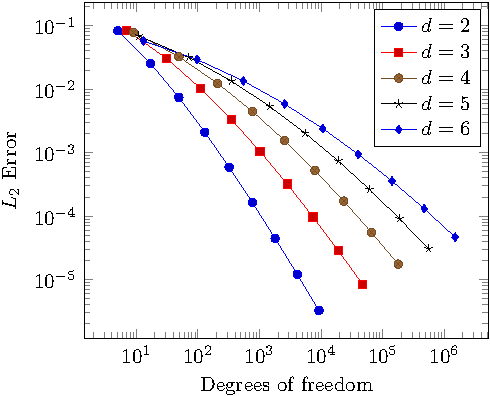
\includegraphics[width=0.95\columnwidth]{figures/example2.pdf}
  \caption{Example of a simple single-column figure. Don't put this
    too early in the document since we don't want it to go in the
    first column.}
  \label{fig:simple}
\end{figure}




%----------------------------------------------------------

\bibliography{rmxac}

%----------------------------------------------------------

\end{document}
\section{Preamble}
        
        The first line to appear in your document should be 
        
        \bigskip
        \CS{documentclass}\verb+{rmaaSC_rho}+
        
        \bigskip
        or
        
        \bigskip
        \CS{documentclass}[\textbf{optionlist}]\verb+{rmaaSC_rho}+
        
        \bigskip
        \noindent which sets up the document to use the rmaaSC class, using the default \texttt{manuscript} option, which is designed for use by authors who submit articles to the Main RMxAA journal. The following commands can be used after the \CS{documentclass} command, but before \CS{begin}$\{\mathrm{document}\}$.
        
        \subsection{Title}
        
        The \CS{title} command defines the title of the article. The title text should be entered in mixed case. In general, for archival and reference purposes, it is recommended not to use mathematical expressions in a title, but they are allowed. 
        
        \bigskip
        \CS{documentclass}\verb|{title text}|
        
        \bigskip
        
        \subsection{Author information}
        
        The \CS{author} command defines the authors of the article. In addition to this command, the \CS{affil} command can be used to define the affiliation of the authors. This will be typed below the authors’ names. Individual authors should be entered in the style \texttt{A.\~{}B.\~{}Lastname} to avoid line breaks within the name. Line breaks may be inserted by hand using a double backslash symbol “\CS \CS". If the authors have various affiliations, you can put more than one of them in the square bracket preceding the author name, as in the example.
        
        \bigskip
        \CS{author}[\textbf{affil list}]\verb|{author name text}|
        
        \bigskip
        and
        
        \bigskip
        \CS{affil}[\textbf{number or symbol}]\verb|{affiliation text}|
        